% \iffalse
\let\negmedspace\undefined
\let\negthickspace\undefined
\documentclass[journal,12pt,twocolumn]{IEEEtran}
\usepackage{cite}
\usepackage{amsmath,amssymb,amsfonts,amsthm}
\usepackage{algorithmic}
\usepackage{graphicx}
\usepackage{textcomp}
\usepackage{xcolor}
\usepackage{txfonts}
\usepackage{listings}
\usepackage{enumitem}
\usepackage{mathtools}
\usepackage{gensymb}
\usepackage{comment}
\usepackage[breaklinks=true]{hyperref}
\usepackage{tkz-euclide} 
\usepackage{listings}
\usepackage{gvv}                                        
\def\inputGnumericTable{}                                 
\usepackage[latin1]{inputenc}                                
\usepackage{color}                                            
\usepackage{array}                                            
\usepackage{longtable}                                       
\usepackage{calc}                                             
\usepackage{multirow}                                         
\usepackage{hhline}                                           
\usepackage{ifthen}                                           
\usepackage{lscape}
\usepackage{placeins}
\usepackage{xparse}


\newtheorem{theorem}{Theorem}[section]
\newtheorem{problem}{Problem}
\newtheorem{proposition}{Proposition}[section]
\newtheorem{lemma}{Lemma}[section]
\newtheorem{corollary}[theorem]{Corollary}
\newtheorem{example}{Example}[section]
\newtheorem{definition}[problem]{Definition}
\newcommand{\BEQA}{\begin{eqnarray}}
\newcommand{\EEQA}{\end{eqnarray}}
\newcommand{\define}{\stackrel{\triangle}{=}}
\theoremstyle{remark}
\newtheorem{rem}{Remark}

\graphicspath{ {./figs/} } 

\begin{document}

\bibliographystyle{IEEEtran}
\vspace{3cm}

\Large\title{GATE 2022 EE 28}
\large\author{EE23BTECH11032 - Kaustubh Parag Khachane $^{*}$% <-this % stops a space
}
\maketitle
\newpage
\bigskip

\renewcommand{\thefigure}{\theenumi}
\renewcommand{\thetable}{\theenumi}
\large\textbf{Question GATE 22 EE 28} :\\
The network shown below has a resonant frequency of 150 kHz and a bandwidth of
600 Hz. The $Q$-factor of the network is \rule{1cm}{0.15mm}
\begin{figure}[!ht]
\centering
\begin{center}
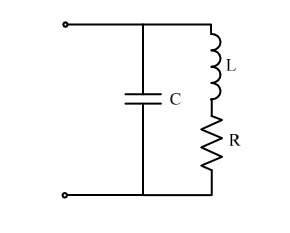
\includegraphics[width=\columnwidth]{question}
\end{center}
%\caption{Diagram for GATE ME Question 30}
\end{figure}
\hfill(GATE EE 2022)\\
\solution\\
\begin{table}[!ht] 
\centering
\setlength{\extrarowheight}{8pt}
\begin{tabular}{|l|l|l|}
    \hline
    \textbf{Parameter} & \textbf{Description} & \textbf{Value} \\
    \hline
     m & Mass of object & 10 Kg \\\hline
     $\mu$ & Frictional coefficient \brak{static} & 0.25\\\hline
     x\brak{t} & Displacement of block &  \\\hline
     $x\brak{0}$ & Initial displacement & 0 \brak{assumed} \\\hline
     g & Gravitational acceleration & 10 $m/s^2$ \\\hline
     $F_s$ & Spring force &  \\\hline
     f & frictional force &  $\mu$ N \\\hline
     N & Normal Force & mg $cos\brak{\theta}$ \\\hline
    \end{tabular}
  \vspace{4mm}
 \caption{Parameter Table}
 \label{tab:table0_xe80}
\end{table}

In the state of resonance ,
\begin{align}
    \omega_0 &= \frac{1}{\sqrt{LC}}\label{eq:eq1}\\
    f_0 &= \frac{1}{2\pi \sqrt{LC}}
\end{align}
Bandwidth is range of frequencies where power is $\geq$ maximum power.\\
Hence it is the range of frequencies between the two points where power is half.\\
\begin{align}
    \text{Power is half }\implies I = \frac{I_0}{\sqrt{2}}
\end{align}
Current at any point is given by ,
\begin{align}
    \frac{V}{\sqrt{R^2 + \brak{\omega L - \frac{1}{\omega C}}^2}} = \frac{V}{R\sqrt{2}}
\end{align}
Solving the above equation, we will get two solution $\omega_1$ and $\omega_2$ which will satisfy
\begin{align}
    \brak{\omega L - \frac{1}{\omega C}} &= \pm R\\
    \implies \omega_2 - \omega_1 = \frac{R}{L}\\
    \therefore \text{Bandwidth } = \frac{R}{L} \label{eq:eq2}
\end{align}
\begin{align}
    Q \text{ factor } &= 2\pi\frac{\text{Peak energy stored}}{\text{Energy disspated in one cycle}} \\
    &= \frac{\frac{1}{2}LI^2}{\frac{1}{2} I^2R\frac{1}{f_0}}\\
    &= \frac{\omega_0}{\frac{R}{L}}\\
\end{align}
Using equations \eqref{eq:eq1} and \eqref{eq:eq2},
\begin{align}
    Q &= \frac{150000}{600}\\
    &= 250
\end{align}
\end{document}
